\section{Subroutines \& Stack}

\subsection{Stack}

\begin{wrapfigure}{l}{0.2\textwidth}
    \centering
    \hspace{-20pt}
    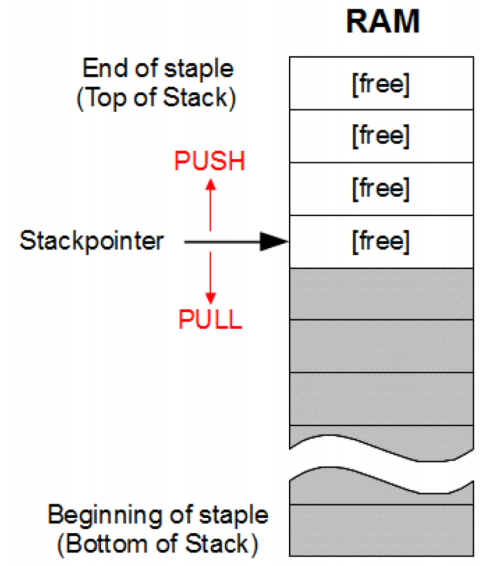
\includegraphics[width=0.2\textwidth]{stack-commands.png}
    \hspace{-50pt}
\end{wrapfigure}

\textit{
    The stack is a special memory section (in RAM)
    that works after the Last-In-First-Out (\textbf{LIFO})
    principle.
    \newline
    It is addressed over the Stackpointerregister
    \textbf{SP} of the CPU.
    \newline
    \textbf{PUSH} put and increment SP
    \newline
    \textbf{PULL} get and decrement SP
    \newline
    Stack grows from high addresses to lower
}

\begin{lstlisting}
Stacksize: EQU $40
             :
DATA:      SECTION
TofStack:  DS Stacksize-1 ; reserve stack
BofStack:  DS 1
             :
PROGRAM:   SECTION
           LDHX #(BofStack+1) ; H:X := Bottom of Stack
           TXS                ; SP := HX -1
             :
           ; save CPU-Status on stack
           PSHA ; Akku auf Stack
           PSHX ; X-Register auf Stack
             :
           ; restore CPU-Status from stack
           ; order is imporant (LIFO!)
           PULX ; X-Register
           PULA ; Akku
\end{lstlisting}

\textit{Stacks are used for:}

\begin{itemize}
    \item{\textit{Subroutine calls (save return address)}}
    \item{\textit{Store context}}
    \item{\textit{Store parameters}}
    \item{\textit{Store local variables}}
\end{itemize}

\textit{malloc (heap) and global variables are not stored on the stack.}

\subsection{Subroutines}

\begin{wrapfigure}{l}{0.2\textwidth}
    \centering
    \hspace{-20pt}
    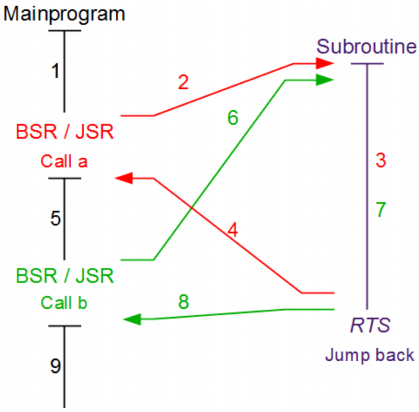
\includegraphics[width=0.2\textwidth]{subroutines.png}
    \hspace{-50pt}
\end{wrapfigure}

\textit{
    \newline
    \textbf{BSR/JSR} push and inc. PC \newline
    \textbf{RTS} pull and inc. PC \newline
    \textbf{Parameters} passing on stack (used by C) \newline
    \textbf{Local Variables} saved on stack (used by C) \newline
    \newline
    \newline
}

\textit{subroutines enable following:}

\begin{itemize}
    \item{\textbf{less memory usage}; repeated command sequences are stored only once}
    \item{\textbf{less development effort}; tested command sequences can be reused}
    \item{\textbf{less error prone}; enable modular way of building software}
    \item{\textbf{higher team productivity}; multiple people can work parallel on different code sections}
    \item{\textbf{shorter compile time \& libraries}; different parts of the code can be compiled seperatly}
\end{itemize}

\textit{
    The only \textbf{negative} about subroutines is calling of subroutines is
    \textbf{slower}. Time is needed for passing parameters and saving the context
    on the stack
}

\subsection{Stack size}

\textit{
    To analyze the used stack size, it is helpful to create a tree with
    the subroutines, their calls and used stack space.
}

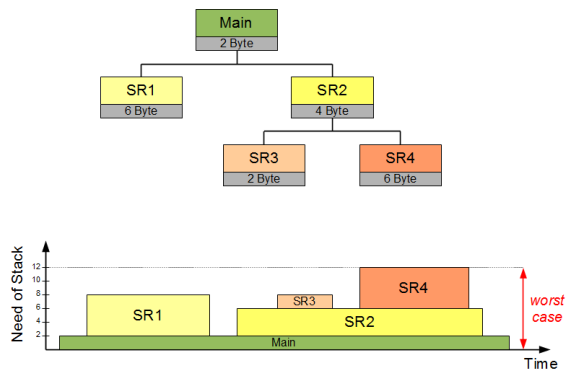
\includegraphics[width=0.5\textwidth]{stack-nested-tree.png}

\textit{
    It is also possible to figure out the stack usage by filling the
    program-stack at the start with an bit pattern like 0xdeadbeef and
    stress test the program as much as possible.
    At the end, this will show which part and how much of the stack has been
    used during the program execution.
}


